% Created 2021-12-16 Thu 20:49
% Intended LaTeX compiler: pdflatex
\documentclass[11pt]{article}
\usepackage[utf8]{inputenc}
\usepackage[T1]{fontenc}
\usepackage{graphicx}
\usepackage{longtable}
\usepackage{wrapfig}
\usepackage{rotating}
\usepackage[normalem]{ulem}
\usepackage{amsmath}
\usepackage{amssymb}
\usepackage{capt-of}
\usepackage{hyperref}
\usepackage{minted}
\usepackage[paper=a4paper,margin=2cm]{geometry}
\usepackage{parskip}
\author{Marc van der Sluys}
\date{\today}
\title{Org mode example}
\hypersetup{
         colorlinks = true,
         linkcolor = black,
         citecolor = black,
         urlcolor = black,
         pdfauthor={Marc van der Sluys},
         pdftitle={Org mode example},
         pdfkeywords={},
         pdfsubject={},
         pdfcreator={Emacs 27.2 (Org mode N/A)}, 
         pdflang={English}
      }
      \author{Marc van der Sluys}
      \begin{document}

\maketitle
\tableofcontents


\section{Key strokes}
\label{sec:orge35717d}
\begin{enumerate}
\item I use lower-case letter \texttt{a} for the \texttt{A}-key.
\item I use upper-case letter \texttt{C-} for the \texttt{Ctrl} key, \texttt{M-} for the Alt (meta) key and \texttt{S-} for the \texttt{Shift} key.
\begin{itemize}
\item hence \texttt{C-c} is \texttt{Ctrl-C}, \texttt{C-c C-c} is twice that and \texttt{C-M-a} means simultaneously press \texttt{Ctrl}, \texttt{Alt} and
\texttt{A}.
\item note that you can type e.g. \texttt{C-c C-x C-l} without releasing the \texttt{Ctrl} key (i.e., keep \texttt{Ctrl} pressed
while typing \texttt{c x l}).
\end{itemize}
\item \texttt{ENTER}, \texttt{TAB} and \texttt{ESC} are the keys you'd expect.
\item Got confused?  Press \texttt{ESC ESC ESC} and you should be good to start typing again.
\item See also \url{http://pub.vandersluys.nl/download/GettingStartedWithEmacs.pdf} (in particular section 1.2 and the
start of 1.3)
\end{enumerate}

\section{{\bfseries\sffamily TODO} To do [1/3]}
\label{sec:org35df544}
\subsection{{\bfseries\sffamily DONE} What to use Org mode for [8/8]}
\label{sec:orga78f003}
\begin{enumerate}
\item{$\boxtimes$} note taking, personal wiki, writing documentation
\item{$\boxtimes$} the brainstorm phase of a project, paper:
\begin{enumerate}
\item Overview in Org mode
\item then export to \LaTeX{} to finish
\end{enumerate}
\item{$\boxtimes$} clock tasks, projects
\item{$\boxtimes$} agenda, planning, task lists (TODO/PROGRESS/DONE), issues (OPEN/ASSIGNED/CLOSED), idea lists, \ldots{}
\item{$\boxtimes$} (internal) links
\item{$\boxtimes$} tables, simple spreadsheets
\item{$\boxtimes$} export, publish: plain text (ASCII, UTF-8), html, md, \LaTeX{}/PDF (+Beamer!), odt, reST, \ldots{}
\item{$\boxtimes$} equations, code
\end{enumerate}

\subsection{{\bfseries\sffamily PROGRESS} Add file with simple examples [5/6]}
\label{sec:orgf01a5a2}
\subsubsection{{\bfseries\sffamily DONE} Text style}
\label{sec:orga18de45}
\begin{itemize}
\item \textbf{bold}
\item \emph{italics}
\item \uline{underlined}
\item \sout{strike through}
\item \texttt{code} or \texttt{verbatim}
\end{itemize}

\subsubsection{{\bfseries\sffamily DONE} Task lists and headings [33\%]}
\label{sec:orge7c8c57}
\begin{itemize}
\item[{$\boxtimes$}] see \ref{sec:org35df544}
\item[{$\boxtimes$}] indent:
\begin{itemize}
\item put the cursor on an item (e.g. in this list) and press \texttt{Alt-arrow right/left}
\item same for headers
\end{itemize}
\item[{$\square$}] drag:
\begin{itemize}
\item put the cursor on an item and press \texttt{Alt-arrow up/down}
\item up/down swaps items (with the same indentation and if possible)
\item the same for headers (of the same level)
\end{itemize}
\item[{$\square$}] change list symbols:
\begin{itemize}
\item put the cursor on an item and press \texttt{Shift right/left}
\item symbols change between \texttt{+/-/*/1./1)} (\texttt{*} if possible)
\end{itemize}
\item[{$\boxtimes$}] (de)select item (radio button):
\begin{itemize}
\item put the cursor on the item and press \texttt{C-c C-c}
\item the number or percentage in the parent header (created by typing \texttt{[/]} or \texttt{[\%]}) changes as well
\end{itemize}
\item[{$\square$}] change TODO:
\begin{itemize}
\item put the cursor on a header and press \texttt{Shift right/left}
\item if all subheaders are DONE, the parent header changes from TODO to DONE as well
\end{itemize}
\item[{$\square$}] new item in a list:
\begin{itemize}
\item \texttt{Alt-ENTER}
\end{itemize}
\item[{$\square$}] new header in a document:
\begin{itemize}
\item \texttt{Ctrl-ENTER}
\end{itemize}
\item[{$\square$}] Create new list
\begin{enumerate}
\item Enumerated:
\begin{enumerate}
\item type \texttt{1.} or \texttt{1)} followed by a space and the description
\item press \texttt{Alt-ENTER} for the next item (counts automatically)
\end{enumerate}
\item Bullets (unnumbered):
\begin{enumerate}
\item type a \texttt{+}, \texttt{-} or (if subitem) \texttt{*} followed by a space and the description
\item press \texttt{Alt-ENTER} for the next item with the same symbol
\end{enumerate}
\item Definition:
\begin{description}
\item[{Definition}] a definition is an \textbf{unnumbered} item with a keyword, followed by a double colon (\texttt{::})
and the definition.
\item \texttt{Alt-ENTER} asks for the next definition with the same symbol
\end{description}
\item Check box/Radio button:
\begin{enumerate}
\item type an item symbol or number, followed by a space, \texttt{[ ]}, another space and the description
\item the \texttt{[ ]} lights up to show that the check box is active
\item \texttt{Alt-ENTER} produces a new item, but \textbf{no} empty check box (bug?)
\item \texttt{C-c C-c} on the line toggles between \texttt{[ ]} and \texttt{[X]}
\end{enumerate}
\end{enumerate}
\end{itemize}

\subsubsection{{\bfseries\sffamily DONE} Links}
\label{sec:org0e30ab0}
\begin{itemize}
\item Internal link: see \ref{sec:org35df544}
\item External link: \url{https://github.com/MarcvdSluys/}
\item External link with description: \href{https://github.com/MarcvdSluys/}{My GitHub page}
\end{itemize}

\subsubsection{{\bfseries\sffamily DONE} Table/spreadsheet}
\label{sec:org6462786}
\begin{enumerate}
\item type \texttt{|- TAB} for a horizontal line
\item type \texttt{x|x\textasciicircum{}2|x\textasciicircum{}3 TAB} in the new line for the header
\item type \texttt{-} right against the \texttt{|} for another line
\item in the left column, type \texttt{1 ENTER 2 ENTER} etc.
\item under x\textsuperscript{2}, type \texttt{=\$1**2 TAB}.  \texttt{\$1} represents column 1.
\item under x\textsuperscript{3}, type \texttt{=\$1**3 TAB}
\item go to the line with \texttt{TBLFM} (table formula) under the table and press \texttt{C-c C-c}
\end{enumerate}

\begin{center}
\begin{tabular}{rrr}
\hline
x & x\textsuperscript{2} & x\textsuperscript{3}\\
\hline
1 & 1 & 1\\
2 & 4 & 8\\
3 & 9 & 27\\
4 & 16 & 64\\
5 & 25 & 125\\
\hline
\end{tabular}
\end{center}


\subsection{{\bfseries\sffamily PROGRESS} More advanced examples}
\label{sec:orgcabe173}
\subsubsection{{\bfseries\sffamily DONE} Equations}
\label{sec:org4d2fa87}
\LaTeX{} must be installed to display formatted equations in emacs.

\begin{enumerate}
\item Lazy symbols outside equations using inline \LaTeX, like \(\int\), \(\infty\) and \(\nabla\)\textsubscript{\(\phi\)} will show up nicely
in \LaTeX.

\item inline: type \texttt{\$\textbackslash{}int\_0\textasciicircum{}\textbackslash{}infty \textbackslash{}frac\{\textbackslash{}sin x\}\{x\} dx\$} and press \texttt{C-c C-x C-l} to display in emacs.
This is a nice equation \(\int_0^\infty \frac{\sin x}{x} dx\), but complicated.

\item between the lines: type \texttt{\textbackslash{}[\textbackslash{}int\_0\textasciicircum{}\textbackslash{}infty \textbackslash{}frac\{\textbackslash{}sin x\}\{x\} dx\textbackslash{}]} and press \texttt{C-c C-x C-l} to display in
emacs.
\[\int_0^\infty \frac{\sin x}{x} dx\]
\end{enumerate}

\subsubsection{{\bfseries\sffamily ACTIVE} Code}
\label{sec:org9b5e568}
\begin{itemize}
\item Elisp always works?
\end{itemize}

\begin{enumerate}
\item Elisp (emacs lisp script)
\label{sec:orga86e84b}
\begin{enumerate}
\item press \texttt{C-c C-, s} for a \texttt{\#+begin/end\_src}-block and add \texttt{elisp} yourself
\item type some code and return a value (see example below)
\item in the code block, press \texttt{C-c C-c} and answer the question in the minibuffer below with \texttt{yes ENTER}
\item the result appears in a \texttt{RESULTS} block under the code, a bit like in a Jupyter notebook.
\end{enumerate}
\begin{minted}[breaklines=true,breakanywhere=true]{elisp}
(concat  (emacs-version)
	 "\nOrgmode " (org-version))  
\end{minted}

\begin{verbatim}
GNU Emacs 27.2 (build 1, x86_64-pc-linux-gnu, GTK+ Version 3.24.29, cairo version 1.16.0)
 of 2021-10-01
Orgmode N/A
\end{verbatim}

\item Bash
\label{sec:orgca78b83}
Bash must be installed and Babel must be activated for Bash\ldots{}
\begin{minted}[breaklines=true,breakanywhere=true]{bash}
echo "My home directory is $HOME"
\end{minted}

\begin{verbatim}
My home directory is /home/sluys
\end{verbatim}

\item Python
\label{sec:orgdf23cc6}
Python must be installed and Babel must be activated for Python\ldots{}

\begin{enumerate}
\item press \texttt{C-c C-, s} for a \texttt{\#+begin/end\_src}-block and type \texttt{python} yourself
\item type some code and return a value
\item In the code block, press \texttt{C-c C-c} and answer the question in the minibuffer below with \texttt{yes ENTER}
\item the return value appears below the code in a \texttt{RESULTS} block
\end{enumerate}
\begin{minted}[breaklines=true,breakanywhere=true]{python}
x=3
y=5
z=x*y
return z
\end{minted}

\begin{verbatim}
15
\end{verbatim}



\begin{minted}[breaklines=true,breakanywhere=true]{python}
import numpy as np
import matplotlib.pyplot as plt
x = np.linspace(-15,15)
plt.plot(x, np.sin(x)/x)
plt.savefig('Orgmode_example.png')
return 'Orgmode_example.png'  # Return filename to Org mode
\end{minted}

\begin{center}
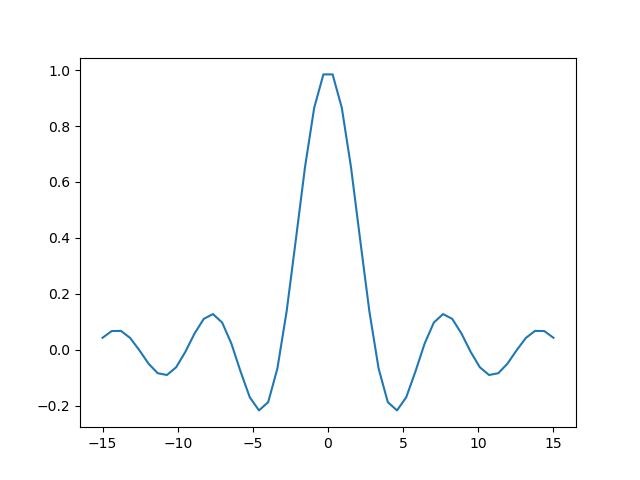
\includegraphics[width=.9\linewidth]{Orgmode_example.png}
\end{center}

\item Python + Bash
\label{sec:orgade0fef}
\begin{itemize}
\item Nicked from \url{https://jherrlin.github.io/posts/emacs-orgmode-source-code-blocks/}
\end{itemize}

Print a list with a selection of files in the current directory in bash.  I will export both (\texttt{both}) the code
and the result (to e.g. \texttt{.md} or \texttt{.pdf}).  Also, I will give the code a name (\texttt{ls}) so that the
output can be used later:
\begin{minted}[breaklines=true,breakanywhere=true]{bash}
ls -lb Orgmode_example.*
\end{minted}

\begin{verbatim}
-rw-r--r-- 1 sluys sluys   9431 Dec 16 20:45 Orgmode_example.md
-rw-r--r-- 1 sluys sluys  37346 Dec 16 20:40 Orgmode_example.odt
-rw-r--r-- 1 sluys sluys   7945 Dec 16 20:48 Orgmode_example.org
-rw-r--r-- 1 sluys sluys 321571 Dec 16 20:45 Orgmode_example.pdf
-rw-r--r-- 1 sluys sluys  23293 Dec 16 20:49 Orgmode_example.png
-rw-r--r-- 1 sluys sluys   9647 Dec 16 20:41 Orgmode_example.rst
-rw-r--r-- 1 sluys sluys  12347 Dec 16 20:45 Orgmode_example.tex
-rw-r--r-- 1 sluys sluys   9178 Dec 16 20:41 Orgmode_example.txt
\end{verbatim}


Use \texttt{awk} to take the file names and sizes from \texttt{ls} and create a table:
\begin{minted}[breaklines=true,breakanywhere=true]{awk}
BEGIN { OFS="|" }; { print $5, $9}
\end{minted}

\begin{center}
\begin{tabular}{rl}
9431 & Orgmode\textsubscript{example.md}\\
37346 & Orgmode\textsubscript{example.odt}\\
7945 & Orgmode\textsubscript{example.org}\\
321571 & Orgmode\textsubscript{example.pdf}\\
23293 & Orgmode\textsubscript{example.png}\\
9647 & Orgmode\textsubscript{example.rst}\\
12347 & Orgmode\textsubscript{example.tex}\\
9178 & Orgmode\textsubscript{example.txt}\\
\end{tabular}
\end{center}

Use Python to o.a. find the smallest and largest file in the table from \texttt{awk}:
\begin{minted}[breaklines=true,breakanywhere=true]{python}
print(table[0])                     # First row of the table as read
print("Number of files: %i"         % len(table))
print("Smallest file:   (%i b) %s"  % tuple(min(table)))
print("Largest file:    (%i b) %s"  % tuple(max(table)))
print("Total size:      %0.3f kb"   % (sum([x for x,y in table]) / 1000))
\end{minted}

\begin{verbatim}
[9431, 'Orgmode_example.md']
Number of files: 8
Smallest file:   (7945 b) Orgmode_example.org
Largest file:    (321571 b) Orgmode_example.pdf
Total size:      430.758 kb
\end{verbatim}
\end{enumerate}
\end{document}
